\problemname{Game Design}

Carol enjoys playing with wooden games. The objective of the game that
fascinates her the most is to tilt a maze, made out of $1\text{ cm}$-by-$1\text{ cm}$ blocks, in
any of the four cardinal directions to move a ball to a hole in the
centre at $(0, 0)$. As shown in Figure~\ref{fig:maze}, once the $1\text{ cm}$ wide ball starts moving, it keeps
going until either it runs into a wooden block, or it falls
into the hole---whichever comes first.

\begin{figure}[h!]
  \centering
  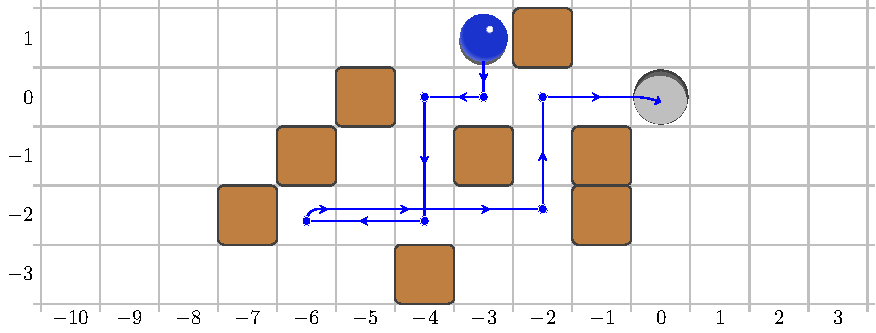
\includegraphics[width=0.96\textwidth]{fig}
  \caption{Illustration of Sample Output 1.}
  \label{fig:maze}
\end{figure}

\vspace{-1mm}

Carol is interested in designing a maze of her own, and like any good
game designer she already has a fixed solution in mind. This is given as a
sequence of tilt moves which must all be followed in order. If any move causes
nothing to happen, for example because the ball is up against a block in that
direction or already in the hole, the solution does not count.

The ball can be placed anywhere to start. Carol will take care of adding a
square border of blocks covering the rows and columns $10^9+1$ cells away from
the centre in each direction.

Design a board which can be won by applying her sequence of moves.

\vspace{-1mm}

\section*{Input}

The input consists of:
\begin{itemize}
    \item One line with a string $s$ consisting of only the characters
          ``\texttt{LRUD}'' ($1 \le |s| \le 20$),
          the sequence of moves. These characters
          correspond to the directions $-x, +x, +y, -y$ respectively.
          No two consecutive characters in $s$ are the same.
\end{itemize}

\vspace{-1mm}

\section*{Output}

If it is possible to create a maze with the given solution,
first output $x$ and $y$, the integer coordinates for the ball to start at.
Then on the next line, output $n$, the number of blocks to use.
On each of the remaining $n$ lines, output $s$ and $t$, the integer coordinates of a block.

Otherwise, output ``\texttt{impossible}''.

You may use at most $n \le 10^4$ blocks. All coordinates
used must be at most $10^9$ in absolute value. No coordinate pair may be the
same as the centre or any other coordinate pair.
If there are multiple valid solutions, you may output any one of them.
